% !TeX spellcheck = english
% !TEX root = thesis.tex
\section{Enhancement of Raman Scattering from Resonant Nanoparticles}

    \subsection{\hlb{Mie-type resonances of dielectric nanoparticles}}
            An important problem for dieletric nanophotnoics is the scattering of eletromagnetic radiation by
        a homogeneous sphere. This problem has an analyticial solution, generally called Mie theory\cite{mie1908beitrage}. The following
        is a condensed version of the solution, following the presentation from Ref. \cite{ng2000manipulation}.
        We will assume an x-polarised incident wave with amplitude $E_0$, propagation constant $\beta_0$ travelling in the $z$ direction:

        \begin{align}
            \vec{E}_{inc} = E_0 e^{i\beta_0z}\hat{x}
        \end{align}

        \subsubsection{\hlb{Maxwell's Equations}}
            Starting with
            \begin{align}
                \nabla \times \vec{E} &= i\omega\mu\vec{H} \\
                \nabla \times \vec{H} &= -i\omega\epsilon\vec{E}
            \end{align}

            Taking the rotor of the equations and substituting,

            \begin{align}
                \nabla \times (\nabla \times \vec{E}) &= i\omega\mu \nabla \vec{H} = \omega^2 \epsilon\mu\vec{E} \\
                \nabla \times (\nabla \times \vec{H}) &= i\omega\epsilon \nabla \vec{E} = \omega^2 \epsilon\mu\vec{H}
            \end{align}

            Applying the vector identity,

            \begin{align}
                \nabla \times \nabla \vec{A} = \nabla (\nabla \cdot \vec{A}) - \nabla \cdot (\nabla\vec{A})
            \end{align}

            We get the following wave equations

            \begin{align}
                \nabla^2\vec{E} + k^2_m\vec{E} &= 0 \label{mie:waveE}\\
                \nabla^2\vec{H} + k^2_m\vec{H} &= 0 \label{mie:waveH}\\
                k^2_m &= \omega^2\epsilon\mu \label{mie:kvec}
            \end{align}

            With $k_m$ as the wave vector in the surrounding medium. The final aim of this derivation is to get vector solutions
            of the wave equations. We begin by
            \begin{itemize}
                \item Transitioning to a spherical coordinate system ${r, \theta, \phi}$, since our system is spherically symmertical
                \item Defining a scalar function $\psi_{l,m}$
                \item Defining a constant vector $\vec{r}$
            \end{itemize}

            The scalar function will be a solution of
            \begin{align}
                \nabla^2\psi + k^2_m\psi = 0 \label{mie:scalar}
            \end{align}

            We can construct three vector solutions:

            \begin{align}
                \vec{L} &= \nabla\psi_{l,m} \\
                \vec{M}_{l,m} &= \nabla\times\vec{r}\psi_{l,m} \\
                \vec{N}_{l,m} &= \frac{1}{k_m}\nabla\times\vec{M}_{l,m}
            \end{align}

            All solutions satisfy the wave equations. $\vec{N}_{l,m}$ and $\vec{M}_{l,m}$ are solenoidal functions and are rotors of each other,
            like $\vec{H}$ and $\vec{E}$. $\vec{L}$, on the other hand is purely longitudal, so we omit it in this analysis.

        \subsubsection{\hlb{Scalar Solution}}

            In spherical coordinates, the scalar solution, $\psi_{l,m}$ of Equation \ref{mie:scalar} is a function of ${R, \theta, \phi}$
            \begin{align}
                \frac{1}{r^2}\frac{\partial}{\partial r}\left(r^2\frac{\partial\psi}{\partial r}\right)
                    + \frac{1}{r^2\sin(\theta)}\frac{\partial}{\partial\theta}\left(\sin(\theta\frac{\partial\psi}{\partial\theta})\right)
                    + \frac{1}{r^2\sin^2(\theta)}\frac{\partial^2\psi}{\partial\phi^2} + k^2_m\psi = 0
            \end{align}

            Next, we seek a solutions that sepratates the variables:

            \begin{align}
                \psi(r,\theta,\phi) &= R(r)\Theta(\theta)\Phi(\phi)
            \end{align}

            Defining constants $m, Q$, we seprate the components into separate solutions:

            \begin{align}
                \frac{d^2\Phi}{d\phi^2} + m^2\Phi &= 0 \\
                (1 - \cos^2(\theta))\frac{d^2\Theta}{d(\cos(\theta))^2} - 2\cos(\theta)\frac{d\Theta}{d(\cos(\theta))}
                    + (Q - \frac{p^2}{1-cos^2(\theta)}) &= 0 \\
                r^2\frac{d^2R}{dr^2} + 2r\frac{dR}{dr} + (k^2_mr^2 - Q^2)R &= 0
            \end{align}

            The solutions to these equations are as follows:

            For $\Phi$
            \begin{align}
                \Phi = e^{\pm i m \phi}
            \end{align}

            For $\Theta$, representing it as an associated Legendre equation:
            \begin{align}
                Q &= l(l+1) \rightarrow \\
                \Theta &= P^m_l(\nu) = \frac{(1-\nu^2)^{\frac{m}{2}}}{2^l l!}\frac{d^{l+m}(\nu^2-1)^l}{d(\nu)^{l+m}} \\
                \nu &= \cos(\theta)
            \end{align}

            From now on, $P_l^m = P_l^m(\nu)$.

            And for $R$
            \begin{align}
                R &= \sqrt{\frac{2}{\pi}}Z_l(p) \\
                p &= k_m r
            \end{align}

            Where $Z_l(p)$ represents the radial spherical Bessl $j_l(p)$ or first order Hankel $h_l(p)$. $h_l(p)$, being infinite in
            the far field are used to represent an outgoing spherical wave pattern for the scattered field. $j_l(p)$ is finite in the
            origin, so it is a correct representation of incident and transmitted fields.

            Combining all of these,

            \begin{align}
                \psi_{l,m}(r, \theta, \phi) = \sqrt{\frac{1}{\pi}}Z_l(k_m r)P_l^m e^{im\phi}
            \end{align}

            or, separating into even and odd components:

            \begin{align}
                \psi_{l,m,\substack{e\\ o}}(r, \theta, \phi) = \sqrt{\frac{1}{\pi}}Z_l(k_m r)P_l^m \substack{\cos\\\sin}(m\phi)
            \end{align}

        \subsubsection{\hlb{Vector Solution}}

            Using the previous equation,

            \begin{align}
                \vec{M}_{l,m, \substack{e \\ o}} &= \nabla \times \hat{r}(r \psi_{l, m, \substack{e \\ o }})\\
                \vec{r} &= \hat{r}r
            \end{align}

            By applying the rotor:

            \begin{align}
                \vec{M}_{l,m}(\hat{r}) &= 0 \\
                \vec{M}_{l,m, \substack{e \\ o}} &= \frac{1}{r\sin(\theta)}\frac{d(r\psi)}{d\phi}\hat{\theta} - \frac{1}{r}\frac{d(r\psi)}{d\theta}\hat{\phi} \\
                &= \mp Z_l\frac{P^m_l}{\sin(\theta)}\substack{\sin \\\cos}(m\phi)\hat{\theta} - Z_l\frac{dP^m_l}{d\theta}\substack{\cos \\ \sin}(m\phi)\hat{\phi}
            \end{align}

            And for $\vec{N}_{m,l\substack{e\\ o}}$

            \begin{align}
                \vec{N}_{l,m,\substack{e\\ o}} &= \frac{l(l+1)}{k_mr}\psi_{\substack{e\\ o}}\hat{r}
                    + \frac{1}{k_mr}\frac{d(r\vec{M}_{l,m,\phi})}{dr} \hat{\theta} + \frac{1}{k_m r}\frac{d(r\vec{M}_{l,m,\theta})}{dr}\hat{\phi} \\
                &= \frac{l(l+1)}{k_mr}Z_l P_l^m \substack{\cos\\\sin}(m\phi) \hat{r}
                    + \frac{1}{r}\frac{d(pZ_l)}{dp}\frac{P_l^m}{d\theta}\substack{\cos\\\sin}m\phi\hat{\theta}  \\
                &\mp m\frac{1}{p}\frac{d(pZ_l)}{dr}\frac{P_l^m}{\sin(\theta)}\substack{\sin\\\cos}(m\phi)\hat{\phi}
            \end{align}

            radial $p$ needs to be replaced by $Np$, $N = \frac{N_s}{N_m}$, which is the relative index of the sphere to the surrounding
            medium.


        \subsubsection{\hlb{Incident, Scattered and Internal Fields}}
            We assume, that an arbitrary wave, expressed by $\vec{A}$ can be represented by a linear combination of vector functions:

            \begin{align}
                \vec{A} = \frac{i}{\omega}\sum_{l,m}\left(A_{l,m}\vec{M}_{l,m}+B_{l,m}\vec{N}_{l,m}\right)
            \end{align}

            Since $\vec{M}_{l,m}$ and $\vec{N}_{l,m}$ are solenoidal function that correspond to interdependece of $\vec{H}$ and $\vec{E}$, using $\vec{A}$:

            \begin{align}
                \vec{H}_{inc} &= \frac{1}{i\omega \mu}\nabla \times \vec{A} \\
                &= - \frac{i}{\omega\mu}\sum\left(A_{l,m}(\nabla\times\vec{M}_{l,m}) + B_{l,m}(\nabla\times\vec{N}_{l,m})\right) \\
                &= - \frac{ik_m}{\omega\mu}\sum\left(A_{l,m}\vec{N}_{l,m}+B_{l,m}\vec{M}_{l,m}\right)
            \end{align}

            Similarly,

            \begin{align}
                \vec{E}_{inc} = \frac{k_m}{\omega^2\epsilon\mu}\sum\left(A_{l,m}\vec{M}_{l,m} + B_{l,m}\vec{N}_{l,m}\right)
            \end{align}

            $A_{l,m}, B_{l,m}$ are expansion coefficients for a particular beam:

            \begin{align}
                A_{l,m} = \int M^*_{l,m}\vec{E}_{inc}d\Omega \\
                B_{l,m} = \int N^*_{l,m}\vec{E}_{inc}d\Omega \\
            \end{align}

            Where $\Omega = 4\pi r$ is the enclosed surface area.

            Similarly, the scattered and internal fields can be expanded in terms of $\vec{M}_{l,m}, \vec{N}_{l,m}$:

            \begin{align}
                \vec{E}_{scat}=& \frac{k_m}{\omega^2\epsilon\mu}\sum\left(A_{l,m}a_l\vec{M}_{l,m} + B_{l,m}b_l\vec{N}_{l,m}\right)\\
                \vec{H}_{scat}=&-\frac{k_m}{\omega\mu}\sum\left(A_{l,m}a_l\vec{M}_{l,m} + B_{l,m}b_l\vec{N}_{l,m}\right)\\
                \vec{E}_{int}=&\frac{k_m}{\omega^2\epsilon_{int}\mu}\sum\left(A_{l,m}c_l\vec{M}_{l,m} + B_{l,m}d_l\vec{N}_{l,m}\right)\\
                \vec{H}_{int}=-&\frac{ik_m}{\omega\mu}\sum\left(A_{l,m}c_l\vec{M}_{l,m} + B_{l,m}d_l\vec{N}_{l,m}\right)
            \end{align}

            Where $a_l, b_l$ are scattering coefficients and $c_d, d_l$ are internal field coefficients.

        \subsubsection{\hlb{Mie Coefficients}}

            The Mie coefficients $a_l, b_l, c_l, d_l$ can be determined from boundary conditions on the edge of the sphere.

            \begin{align}
                \left( \vec{E}_{inc} + \vec{E}_{scat} - \vec{E}_{int} \right) \times \vec{r} &= 0 \\
                \left( \vec{H}_{inc} + \vec{H}_{scat} - \vec{H}_{int} \right) \times \vec{r} &= 0
            \end{align}

            or,

            \begin{align}
                E_{inc,\theta} + E_{scat,\theta} &= E_{int, \theta} \\
                E_{inc,\phi} + E_{scat,\phi} &= E_{int, \phi} \\
                H_{inc,\theta} + H_{scat,\theta} &= H_{int, \theta} \\
                H_{inc,\phi} + H_{scat,\phi} &= H_{int, \phi}
            \end{align}

            Which, substiuting the vector spherical harmonics, gives:

            \begin{align}
                j_l(N\xi)c_l + h_l(\xi)b_l&=j_l(\xi)\\
                [N\xi j_l(N\xi)]'c_l+ [\xi h_l(\xi)]'b_l&= [\xi j_l(\xi)]'\\
                Nj_l(N\xi)d_l + h_l(\xi)a_l &= j_l(\xi)\\
                [N\xi j_l(N\xi)]'d_l +N[\xi h_l(\xi)]'a_l &= N[\xi j_l(\xi)]'
            \end{align}

            which gives us the the stanard expressions for the Mie coefficients:

            \begin{align}
                a_l &= \frac{N^2 j_l(N\xi)[\xi j_l(\xi)]' - j_l(\xi)[N\xi j_l(N \xi)]'}{N^2 j_l(N\xi)[\xi h_l(\xi)]' - h_l(\xi)[N\xi j_l(N \xi)]'}\\
                b_l &= \frac{j_l(N\xi)[\xi j_l(\xi)]' - j_l(\xi)[N\xi j_l(N\xi)]'}{j_l(N\xi)[\xi h_l(\xi)]' - h_l(\xi)[N\xi j_l(N\xi)]'}\\
                c_l &= \frac{j_l(\xi)[\xi h_l(\xi)]' - h_l(\xi)[\xi j_l(\xi)]'}{j_l(N\xi)[\xi h_l(\xi)]' - h_l(\xi)[N\xi j_l(N\xi)]'}\\
                d_l &= \frac{Nj_l(\xi)[\xi h_l(\xi)]' - N h_l(\xi)[\xi j_l(\xi)]'}{N^2 j_l(N\xi)[\xi h_l(\xi)]' - h_l(\xi)[N\xi j_l(N\xi)]'}
            \end{align}

        \subsubsection{\hlb{Cross Sections}}
            Scattering and extinction cross sections can be easily computed, knowing the Mie coefficients.

            \begin{align}
                C_{sca} &= \frac{W_{sca}}{I_{inc}} \\
                C_{ext} &= \frac{W_{ext}}{I_{inc}}
            \end{align}

            \begin{align}
                W_{sca} &= \frac{1}{2}\int_0^{2\pi}\int_0^\pi \left(E_{sca} \times H^*_{sca}\right)r^2\sin(\theta)d\theta d\phi \\
                 &= \frac{1}{2}\int_0^{2\pi}\int_0^\pi \left(E_{sca,\theta} \times H^*_{sca,\phi}\right.
                                \left.- E_{sca,\phi} \times H^*_{sca,\theta}\right)r^2\sin(\theta)d\theta d\phi
            \end{align}

            \begin{align}
                W_{ext} &= \frac{1}{2}\int_0^{2\pi}\int_0^\pi \left(E_{inc} \times H^*_{sca}\right)r^2\sin(\theta)d\theta d\phi \\
                 &= \frac{1}{2}\int_0^{2\pi}\int_0^\pi \left(E_{inc,\phi} \times H^*_{sca,\theta}\right.
                                \left.- E_{inc,\theta} \times H^*_{sca,\phi} - E_{sca,\phi} \times H^*_{inc,\theta}
                                               + E_{sca,\theta} \times H^*_{inc,\phi}\right)r^2\sin(\theta)d\theta d\phi
            \end{align}

            Which can be simlified to

            \begin{align}
                C_{sca} &= \frac{2\pi}{k^2_m}\sum_{l=1}^\infty (2l +1)(|a_l|^2 + |b_l|^2)\\
                C_{ext} &= \frac{2\pi}{k^2_m}\Re\sum_{l=1}^\infty (2l +1)(a_l + b_l)\\
                C_{abs} &= C_{ext} - C_{sca}
            \end{align}

    \subsection{\hlb{Raman scattering from crystalline materials}}
            Raman scattering of light from crystalline materials is a versatile method of probing the phonon stucture of the materials.
        A simplisitc classical model of Raman scattering is sufficient to demonstarte the effect and to properly predict many of the
        Raman scattering peaks of semiconductors\cite{peter2010fundamentals}.

        We start with an infinite medium with electric susceptibility $\chi$. For simplicity, let us assume that the medium is isotropic
        and that the susceptibility is scalar. A plane sinusodial wave is present in the medium, inducing sinusodial polarization:
        \begin{align}
            \vec{F}(\vec{r}, t) &= \vec{F}_i(\vec{k}_i, \omega_i)\cos(\vec{k}_i\cdot\vec{r} - \omega_i t) \\
            \vec{P}(\vec{r}, t) &= \vec{P}(\vec{k}_i, \omega_i)\cos(\vec{k}_i\cdot\vec{r} - \omega_i t) \\
            \vec{P}(\vec{k}_i, \omega_i) &= \chi(\vec{k}_i, \omega_i)\vec{F}_i(\vec{k}_i, \omega_i)
        \end{align}

        The lattice has thermal vibrations, quantized into phonons, causing fluctuations in $\chi$. The atomic displacements of a phonon
        can also be expressed as a plane wave, with wavevector and frequency $\vec{q}, \omega_0$:

        \begin{align}
            \vec{Q}(\vec{r}, t) = \vec{Q}(\vec{q},\omega_0)\cos(\vec{q}\cdot\vec{r}-\omega_0 t)
        \end{align}

        These phonons will perturb $\chi$. Assuming the characteristic electronic frequencies, which determine $\chi$ are
        much larger than $\omega_0$, $\chi$ can be assumed to be a function of $\vec{Q}$. At room temperature the
        amplitudes of the vibrations are small when compared to the lattice constant, meaning we can expand $\chi$ as
        a Taylor series of $\vec{Q}$:

        \begin{align}
            \chi(\vec{k}_i, \omega_i, \vec{Q}) = \chi_0(\vec{k}_i, \omega_i) + \frac{\partial\chi}{\partial\vec{Q}}_0\vec{Q}(\vec{r},t) + ...
        \end{align}

        where $\chi_0$ is the unperturbed susceptibility and the second term is the effect of the lattice wave. Knowing this, we
        can express the polarization of the medium with lattice vibrations:

        \begin{align}
            \vec{P}(\vec{r}, t, \vec{Q}) &= \vec{P}_0(\vec{r},t) + \vec{P}_{ind}(\vec{r}, t, \vec{Q}) \\
            \vec{P}_0 &= \chi_0(\vec{k}_i, \omega_i)\vec{F}_i(\vec{k}_i, \omega_i)\cos(\vec{k}_i\cdot\vec{r} - \omega_i t) \\
            \vec{P}_{ind}(\vec{r}, t, \vec{Q}) &= \frac{\partial\chi}{\partial\vec{Q}_0}\vec{Q}(\vec{r},t)
                                                    \vec{F}_i(\vec{k}_i, \omega_i)\cos(\vec{k}_i\cdot\vec{r}-\omega_i t)
        \end{align}

        Such a simplistic description only includes interaction between TO phonons and EM waves, neglecting LO phonons, which
        can interact with EM waves indirectly, through macroscopic EM fields, but at this moment this is not a serious deficiency.

        \begin{align}
            \vec{P}_{ind}(\vec{r}, t, Q) &= \frac{\partial\chi}{\partial\vec{Q}_0}\vec{Q}(\vec{q},\omega_0)\cos(\vec{q}\cdot\vec{r}-\omega_0 t) \nonumber\\
                                                    &\times\vec{F}_i(\vec{k}_i, \omega_i)\cos(\vec{k}_i\cdot\vec{r}-\omega_i t) \\
                        &= \frac{1}{2}\frac{\partial\chi}{\partial\vec{Q}_0}\vec{Q}(\vec{q},\omega_0)\vec{F}_i(\vec{k}_i, \omega_i) \nonumber\\
                        &\cdot \left( \cos((\vec{q} + \vec{k}_i)\cdot\vec{r} + (\omega_0 + \omega_i) t)
                                    + \cos((\vec{q} - \vec{k}_i)\cdot\vec{r} + (\omega_0 - \omega_i) t)) \right)
        \end{align}

        $\vec{P}_{ind}$ contains two sinusodial waves - a Stokes shifted ($\omega_S = \omega_0 - \omega_i, \vec{k}_S = \vec{k}_i - \vec{q}$) and an
        anti-Stokes shifted wave ($\omega_A = \omega_0 - \omega_i, \vec{k}_A = \vec{k}_i - \vec{q}$). This produces Stokes and anti-Stokes scattered
        light, with the difference in frequency from the original wave know as the Raman shift.

        Since in this case both frequency and wavevector are conserved, single-phonon raman scattering probes only zone-center phonons.
        Expanding the Taylor series we can easily move to multiple phonon scattering. For two phonon scattering we get combination
        and difference modes. If the two phonons are identical, then we observe overtone scattering. In this case there is no limit
        on the wavevector of the individual phonons (only that they need to be identical), meaning that overtone Raman probes the
        overall phonon density of states.

        The intensity of the Raman scattering depends on the polarization of the incident radiation, the scattered radiation and the
        types of phonons participating in the scattering.

        \begin{align}
            I_s \propto | \vec{e}_i \cdot \frac{\partial\chi}{\partial\vec{Q}}\vec{Q}(\omega_0)\cdot\vec{e}_s|^2
        \end{align}

        This approximates $\vec{q} = 0$ for single phonon scattering. $\frac{\partial\chi}{\partial\vec{Q}}$ is a third-rank tensor with
        complex components. Introducing $\vec{Q}_n = \vec{Q}/|\vec{Q}|$, a unit vector in the direction of the phonon diplacement, we can
        define a complex second rank tensor,

        \begin{align}
            \hat{R} &= \frac{\partial\chi}{\partial\vec{Q}}\vec{Q}_n \\
            I_s &\propto | \vec{e}_i \cdot \hat{R} \cdot\vec{e}_s|^2
        \end{align}

        $\hat{R}$ is tha Raman tensor, whose symmetry determines the symmetry of the material's Raman-active phonons. The symmetry of the
        Raman tensor depends on the symmetry of the medium and the active phonons.

    \subsection{\hlb{Enhancement of Raman signal by Mie resonances of nanoparticles\cite{dmitriev2016resonant}}}
        \label{sec:Theory}
            To describe the enhancement of Raman scattering and analyze the role of the electric and magnetic
        Mie resonances of a silicon nanoparticle, we employ the rigorous Green tensor approach. Ideologically,
        our theoretical approach is based on earlier related studies~\cite{canccado2014theory, murphy1983enhanced}.

        In this framework, we first determine the spatial field distribution $\mathbf{E}_{exc}(\mathbf{r})$
        inside the nanoparticle at the excitation frequency created by an external source. Assuming that a
        spherical nanoparticle in free space is illuminated by a plane wave, we represent the normalized
        electric field inside the nanoparticle as a series of vector spherical harmonics~\cite{bohren1983absorption}:
        %
        \begin{align}
            \mathbf{E}_{exc}(\mathbf{r})=\sum\nolimits_{n=1}^\infty E_n \left(c_n\mathbf{M}_{o1n}^{(1)}(\mathbf{r}) -
            i{d_n}\mathbf{N}_{e1n}^{(1)}(\mathbf{r})\right) ,
            \label{eq1}
        \end{align}
        %
        where $c_n$ and $d_n$ are the Mie coefficients, ${{\mathbf{M}}_{o1n}^{(1)}}$ and ${{\mathbf{N}}_{e1n}^{(1)}}$ are
        the orthogonal vectorial spherical harmonics, and ${E_n} = {i^n}(2n + 1)/[n(n + 1)]$. The excitation field distribution
        at each point inside the medium defines the Raman polarization oscillating at the Stokes frequency $\omega_S$ according to
        %
        \begin{align}
            {{\bf{P}}_s}\left( {\bf{r}} \right) = {\chi _s}\hat \alpha_j \left( {\bf{r}} \right){{\bf{E}}_{exc}}\left( {\bf{r}} \right),
            \label{eq2}
        \end{align}
        %
        where $\chi_s$ is the scalar Raman susceptibility, and $\hat \alpha_j$ is the Raman polarizability tensor representing
        the threefold degenerate transverse optical (TO) phonon mode excitation~\cite{ralston1970spontaneous, peter2010fundamentals}.
        Induced Raman polarization, in turn, produces an electromagnetic field at the observation point
        $\mathbf{r}_0$ given by $\mathbf{E}_s(\mathbf{r}_0) = (\omega_s^2/c^2)\int\limits_V {{{\hat G}_s}\left( {{{\mathbf{r}}_0},{\mathbf{r}}} \right){{\mathbf{P}}_s}\left( {\mathbf{r}} \right){d^3}{\mathbf{r}}}$,
        where  ${\hat G_s}\left( {{{\mathbf{r}}_0},{\mathbf{r}}} \right)$ is the Green tensor at the Stokes frequency accounting
        for the Si nanoparticle and integration is carried out over the nanoparticle volume $V$. Finally, the collected signal at
        the point $\mathbf{r}_0$ is presented in the form:
        %
        \begin{align} %Final collected signal
            %\begin{gathered}
                  S\left( {{{\mathbf{r}}_0}} \right) = \sum\limits_j {\left\langle {{\mathbf{E}}_s^*\left( {{{\mathbf{r}}_0}} \right){{\mathbf{E}}_s}\left( {{{\mathbf{r}}_0}} \right)} \right\rangle }  = \sum\limits_j {\frac{{\omega _s^4}}
                {{{c^4}}}\iint\limits_V {{d^3}{{\mathbf{r}}_1}{d^3}{{\mathbf{r}}_2}\left\langle {\hat G_s^*\left( {{{\mathbf{r}}_0},{{\mathbf{r}}_1}} \right){\mathbf{P}}_s^*\left( {{{\mathbf{r}}_1}} \right){{\hat G}_s}\left( {{{\mathbf{r}}_0},{{\mathbf{r}}_2}} \right){{\mathbf{P}}_s}\left( {{{\mathbf{r}}_2}} \right)} \right\rangle }}  \\
                   = \sum\limits_j {\frac{{\omega _s^4}}
                {{{c^4}}}\iint\limits_V {{d^3}{{\mathbf{r}}_1}{d^3}{{\mathbf{r}}_2}\hat G_s^*\left( {{{\mathbf{r}}_0},{{\mathbf{r}}_1}} \right){\mathbf{E}}_{exc}^*\left( {{{\mathbf{r}}_1}} \right){{\hat G}_s}\left( {{{\mathbf{r}}_0},{{\mathbf{r}}_2}} \right){{\mathbf{E}}_{exc}}\left( {{{\mathbf{r}}_2}} \right)\chi _s^2\left\langle {\hat \alpha _j^*\left( {{{\mathbf{r}}_1}} \right) \otimes {{\hat \alpha }_j}\left( {{{\mathbf{r}}_2}} \right)} \right\rangle }},  \\
            %\end{gathered}
            \label{eq4}
        \end{align}
        %
        where summation is performed over the three degenerate TO phonon modes. Since the Raman scattering is a spontaneous process
        (until we enter the stimulated Raman scattering regime), the  induced polarization $\mathbf{P}_s$ is not coherent across
        the whole particle. Therefore, in Eq.~(\ref{eq4}), the averaging is carried out over all possible realizations of the Raman
        polarization $\mathbf{P}_s$. Taking into account that the correlation length of the Raman scattering in silicon $L_c$ is of
        the order of tens nanometer and much less than the nanoparticle diameter, we approximate the correlation of the Raman
        polarizability tensors by the Dirac delta function
        $\left\langle {\hat \alpha_j \left( {{{\mathbf{r}}_1}} \right) \otimes \hat \alpha_j \left( {{{\mathbf{r}}_2}} \right)} \right\rangle \sim \delta \left({{\mathbf{r}_1} - {\mathbf{r}_2}} \right)$.
        Under this assumption, Eq.~(\ref{eq4}) reduces to
        %
        \begin{align}
            S\left( {{{\bf{r}}_0}} \right) = \frac{{\omega _s^4}}{{{c^4}}}\sum\limits_j {\int\limits_V {{d^3}{\bf{r}}{{\left| {{{\hat G}_s}\left(
            {{{\bf{r}}_0},{\bf{r}}} \right){{\hat \alpha }_j}{\chi _s}{{\bf{E}}_{exc}}\left( {\bf{r}} \right)} \right|}^2}} }
            \label{eq5}
        \end{align}
        %
        \begin{figure}[h!]
            \begin{center}
                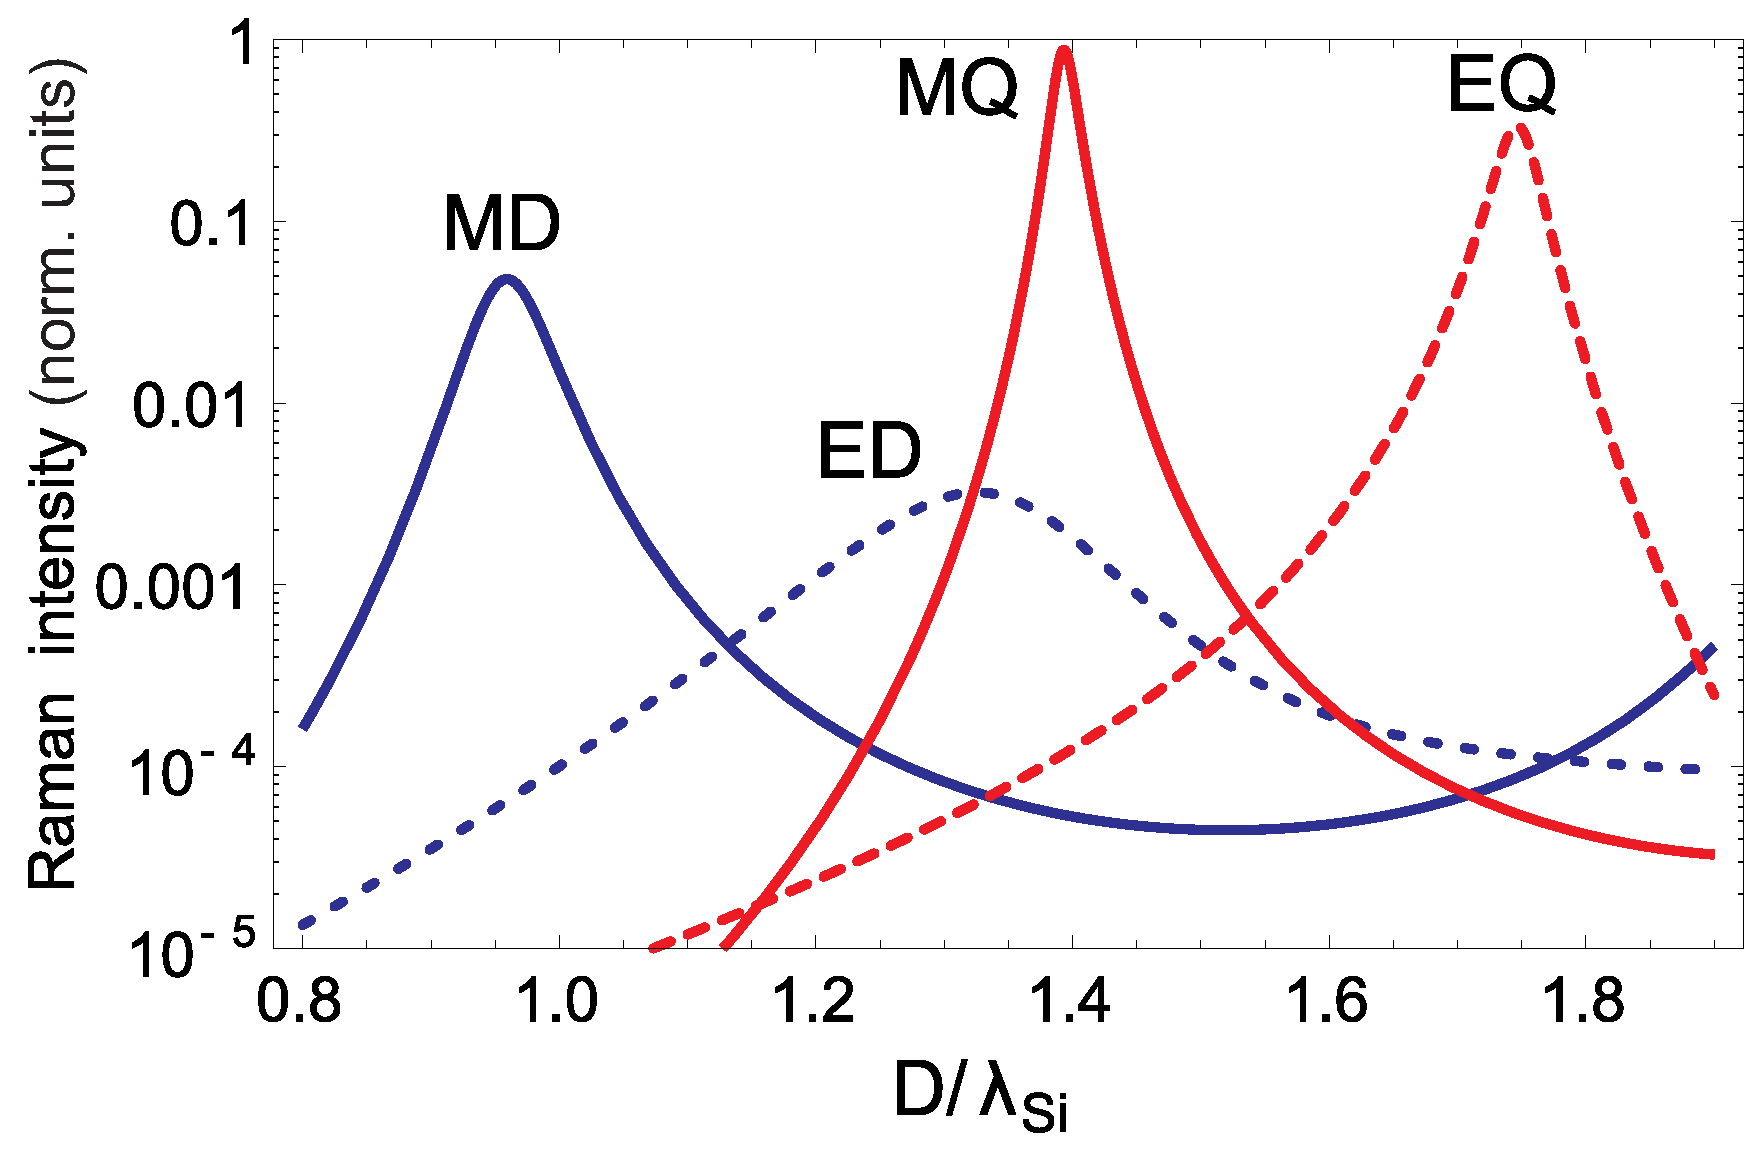
\includegraphics[width=0.5\textwidth]{figs/intro/TheoryEnhancement.eps}
            \end{center}
            \label{fig:TheoryEnhancement}
            \caption{Log plot of normalized intensity of Raman scattering as a function of dimensionless nanoparticle diameter for the magnetic dipole (MD),
            electric dipole (ED), magnetic quadrupole (MQ) and electric quadrupole (EQ) resonances.}
        \end{figure}

            Expression~(\ref{eq5}) can be simplified with the use of the single-mode approximation. First, we notice that the
        electromagnetic response of an optically small Si nanoparticle at the excitation wavelength is dominated by a single
        magnetic or electric multipole resonance depending on the particle radius~\cite{evlyukhin2010optical}. Therefore, we can keep
        only one resonant term in Eq.~(\ref{eq1}) and represent the electric field inside the nanopartice as ${
        {\mathbf{{E}}}_{exc}} \approx {E_n}{c_n}{\mathbf{M}}_{o1n}^{(1)}$, for the $n-$th magnetic resonance, and
        ${{\mathbf{{E}}}_{exc}}\approx -i{E_n}{d_n}{\mathbf{N}}_{e1n}^{(1)}$, for the $n-$th electric resonance,
        respectively. Furthermore, since the Raman shift in silicon is small compared to the linewidth $\gamma$ of
        Mie resonance at $\omega_0$, the main contribution to the Green tensor is provided by the same eigenmode of
        the system. Therefore, expanding the Green tensor in the series of eigenmodes~\cite{ishimaru1991electromagnetic} and keeping only
        the resonant term, we obtain
        %
        \begin{align}
            {\hat G_s}\left( {{{\bf{r}}_0},{\bf{r}}} \right) \approx \frac{{{c^2}}}{{{N^2}}}\frac{{{\bf{u}}\left( {{{\bf{r}}_0}} \right) \otimes
            {\bf{u}}^*\left( {\bf{r}} \right)}}{{{{\left( {{\omega _0} + i\gamma } \right)}^2} - \omega _s^2}},
            \label{eq8}
        \end{align}
        %
        where ${{\mathbf{u}}\left( {{\mathbf r}} \right)}$ is the spatial field distribution of the eigenmode, and
        ${N^2} = {\int {{\mathop{\rm Re}\nolimits} \varepsilon \left( {\bf{r}} \right)\left| {{\bf{u}}\left( {\bf{r}} \right)} \right|} ^2}{d^3}{\bf{r}}$
        is the normalization constant. Finally, integrating the expression (5) over the whole volume $V$ of the nanoparticle, we
        arrive at the following simple expression describing the Raman signal enhanced by a single Mie resonance:
        %
        \begin{align}
            S\left( {{{\mathbf{r}}_0}} \right) \approx V{\left( {\frac{{{\omega _s}}}{c}} \right)^4}{\left| {\frac{{{\chi_s s_n}}}{{{{\left( {{\omega
            _0} + i\gamma } \right)}^2} - \omega _s^2}}} \right|^2},
            \label{eq9}
        \end{align}
        %
        where $s_n$ stands for the Mie coefficient, either $c_n$ or $d_n$ of the corresponding mode. The above expression clearly
        shows that the total enhancement of Raman scattering depends on two factors: the enhancement of the excitation field
        inside the medium, and the Purcell enhancement of the Raman dipoles radiation~\cite{checoury2010deterministic}.

        The two key parameters entering Eq.~(\ref{eq9}) are the resonance frequency $\omega_0$ and the resonance linewidth $\gamma$.
        The resonance frequency can be easily estimated numerically, while for the estimation of the resonance linewidth one can
        employ analytical expressions from Ref.~\cite{lai1991effect}. Substituting these values into Eq.~(\ref{eq9}), we obtain the desired
        spectrum of Raman scattering enhanced by the resonances of a silicon sphere. This spectrum (normalized by the particle
        volume $V=4\pi R^3/3$) is plotted in Fig.~\ref{fig:TheoryEnhancement} as a  function of dimensionless nanoparticle diameter $D/\lambda_{\rm Si}$
        with $\lambda_{\rm Si}=163$~nm being the wavelength of the excitation signal inside the silicon for the magnetic dipole (MD), electric dipole (ED),
        magnetic quadrupole (MQ) and electric quadrupole (EQ) resonances assuming a constant excitation wavelength of 633~nm,
        used below in experiments.

        The derived single-mode expression (\ref{eq9}) allows us to clearly separate contributions of each Mie resonance of the
        nanoparticle into the total Raman scattering enhancement. As follows from Fig.~(\ref{fig:TheoryEnhancement}), the strongest enhancement
        is associated with the MQ resonance due to its high $Q-$factor. Notably, the predicted Raman scattering enhancement
        at the MD resonance, which occurs for the smallest particles, is more than an order of magnitude larger than that for
        the ED resonance.
